% -*-coding: utf-8 -*-
% Держать в начале каждого файла!

\documentclass[a4paper, 12pt]{extarticle}
\usepackage{metod}

\MTDSetPhysSection{Механика}
\MTDSetTitle{Определение ускорения свободного падения с помощью машины Атвуда}
\MTDDesignator{М--1}
\MTDSetGrade{10}

\MTDSetAuthors{И.~Н.~Грачева, В.~И.~Гребенкин, А.~Е.~Иванов, И.~А.~Коротова,
Е.~И.~Красавина, А.~В.~Кравцов, Н.~С.~Кулеба, Б.~В.~Падалкин,
Г.~Ю.~Шевцова, Т.~С.~Цвецинская}

\MTDSetEditorsGenCase{И.~Н.~Грачевой, А.~Е.~Иванова, А.~В.~Кравцова}


\begin{document}

\MTDTitlePage
\MTDInfoPage

\setcounter{section}{1}

\subsection{Цель работы}
Целями работы являются экспериментальное определение значения ускорения свободного падения и экспериментальная проверка уравнения прямолинейного равноускоренного движения точечного тела.

\subsection{Основные теоретические сведения}
При свободном падении точечного тела с некоторой высоты $h$ (начальная скорость равна нулю) уравнение движения тела имеет вид: %ИЗМ: двоеточие
\begin{equation}
\label{eq:m1-free-fall-h}
h = \frac{gt^2}{2}.
\end{equation}

Из этого уравнения по известным $h$ и $t$ определяется ускорение свободного падения $g$: %ИЗМ: двоеточие ИЗМ: "при известных" -> "по известным"
\begin{equation}
\label{eq:m1-free-fall-g}
g = \frac{2h}{t^2}.
\end{equation}

\subsection{Описание экспериментальной установки и методика проведения работы}
\begin{wrapfigure}{l}{0.59\textwidth} 
\centering
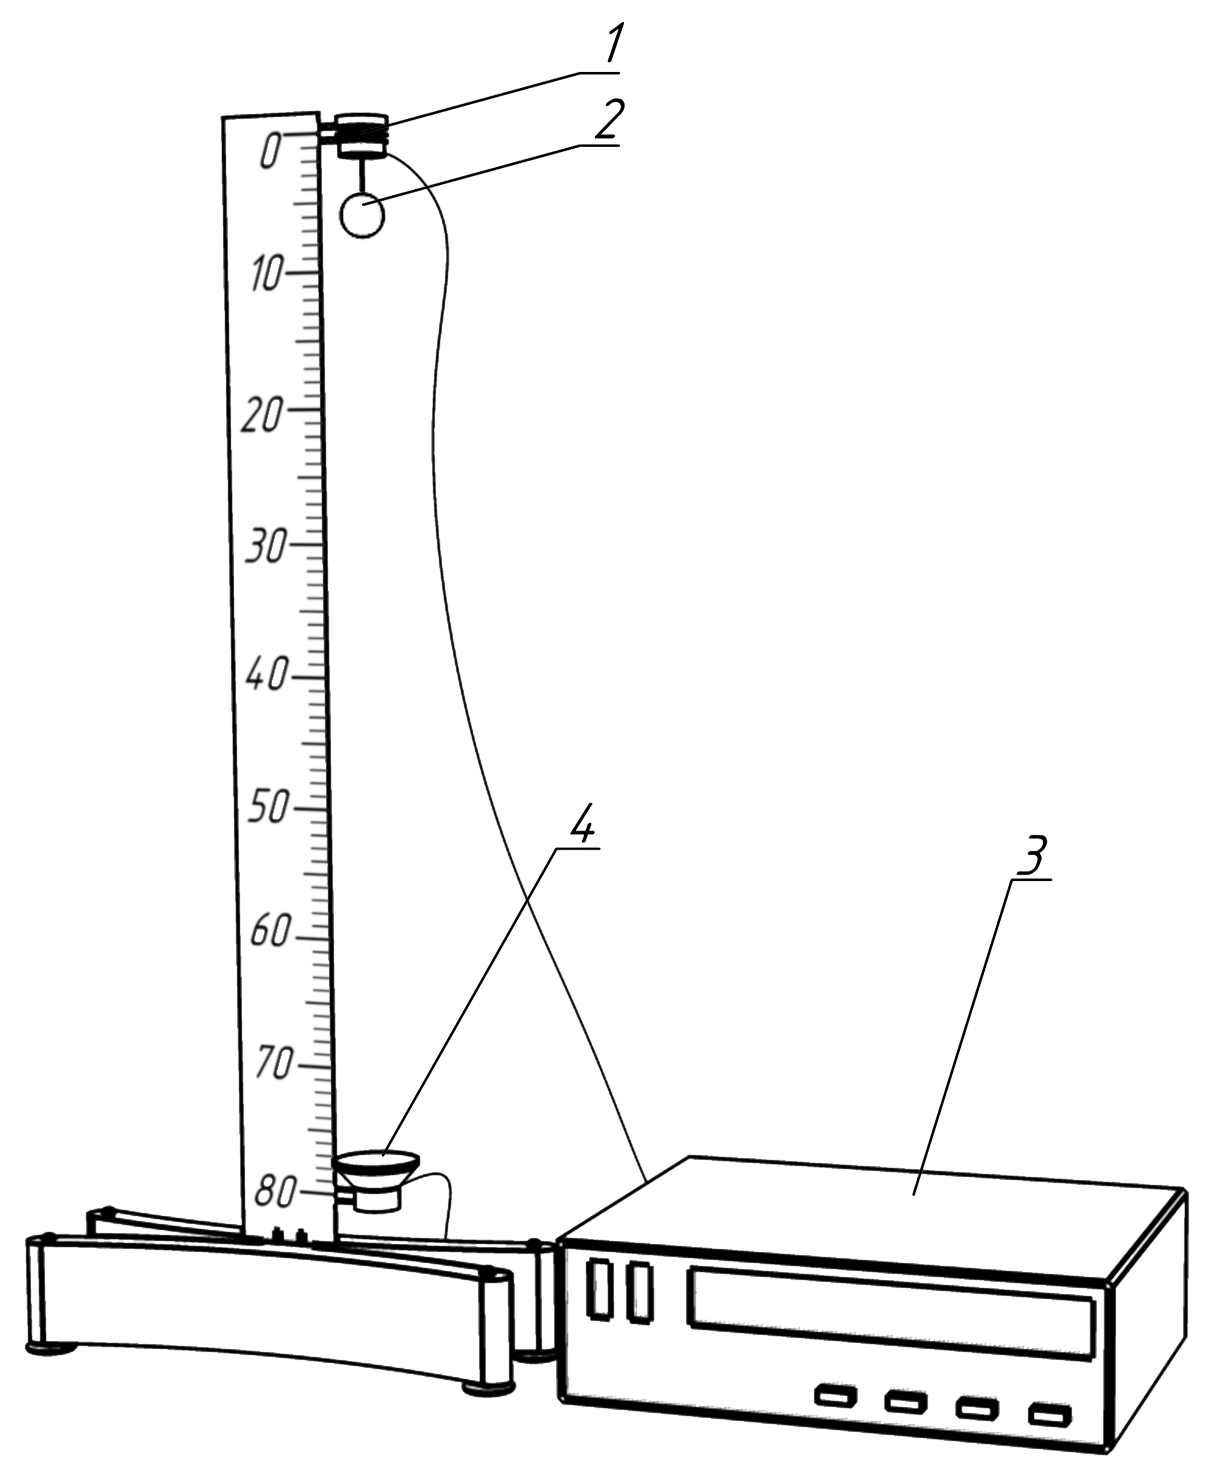
\includegraphics{M1-AtwoodsMachine}
\caption{Схема экспериментальной установки \label{fig:m1-atwood-machine}}
\end{wrapfigure}
Работа выполняется на машине Атвуда с электронным секундомером. Схема установки представлена на рис.~\ref{fig:m1-atwood-machine}.

При замыкании электрической цепи электромагнит~\emph{1} удерживает стальной шарик~\emph{2} на конце иглы~\emph{6}. При разрыве цепи питания (отключении выключателя, находящегося на пульте секундомера~\emph{3}) шарик отрывается и начинает свободно падать, при этом включается секундомер. %мб цифры сделать курсивом?

Приемная площадка~\emph{4} оборудована контактами, формирующими сигнал <<Стоп>> секундомера. Поэтому при ударе шарика о площадку секундомер прекращает отсчет времени. При проведении опытов следует учитывать, что работа приемной площадки в значительной степени зависит от того, насколько тщательно выставлена стойка машины Атвуда в вертикальное положение. Если шарик попадает в центр площадки, то секундомер останавливается практически мгновенно. Для установки стойки служат уравнительные винты~\emph{5}. %ИЗМ: ",следовательно при попадании шарика на площадку" -> ". При ударе шарика о площадку"; ИЗМ: "секундомер включается" -> "секундомер останавливается"

\subsection{Порядок выполнения работы и обработки результатов}
\begin{enumerate}
\item Во время домашней подготовки сделайте таблицу~\ref{tab:m1-res-exp} для записи результатов измерений и вычислений.

\begin{table}[t] %не знаю что с этой таблицей делать: куда и как ее вставлять
\caption{\label{tab:m1-res-exp}}
\begin{center}
\begin{tabular}{|c|c| >{\centering\arraybackslash} m{0.7cm}|>{\centering\arraybackslash} m{0.7cm}|>{\centering\arraybackslash} m{0.7cm}|c|c|c|}
\hline
\multirow{2}*{\textnumero \ измерения} & \multirow{2}*{$h$,~\Units{м}} & \multicolumn{3}{c|}{$t$,~\Units{c}} &\multirow{2}*{\hspace{3pt}$\MTDMean{t},$~\Units{c}} & \multirow{2}*{\hspace{3pt}$\MTDMean{t}^2,~\Units{\text{c}^2}$} & \multirow{2}*{$g,~\Units{\text{м}/\text{c}^2}$} \\ \cline{3-5} % не знаю, нужен ли тут неразрывный
   &  & 1 & 2 & 3 & & & \\ \hline
1 & 0,1 & & & & & & \\ \hline
2 & 0,2 & & & & & & \\ \hline
3 & 0,3 & & & & & & \\ \hline
4 & 0,5 & & & & & & \\ \hline
5 & 0,8 & & & & & & \\ \hline
\end{tabular}
\end{center}
\end{table}

\item Ознакомьтесь с устройством прибора и получите допуск к работе у преподавателя.
\item Приемную площадку укрепите на шкале против отметки 0,8~\Units{м}. Площадка должна быть расположена таким образом, чтобы против отметки находилась верхняя кромка прижимной планки.
\item Установите стойку машины в вертикальное положение.
\item Включите цепь электромагнита и установите шарик на конце иглы. Нажмите кнопку <<Сброс>> секундомера.
\item Выключателем на панели секундомера разомкните цепь электромагнита. Шарик начнет падать, одновременно начнется отсчет времени секундомером. Приборная погрешность секундомера $t = 10^{-4}~\text{\Units{с}}$. При попадании шарика на приемную площадку отсчет времени прекращается. Если шарик не попал в центр приемной площадки, то подрегулируйте винтами~\emph{5} положение стойки и снова повторите пп.~5--6. %ИЗМ п.п. -> пп.
\item Выполняя пп.~5--6, проведите опыты для значений высоты $h$, указанных в таблице~\ref{tab:m1-res-exp}. Для каждой высоты измерения выполняются по 3~раза. Данные измерений занесите в таблицу~\ref{tab:m1-res-exp}. Выполните расчеты и заполните все графы таблицы~\ref{tab:m1-res-exp}. Расчет $g$ следует выполнять по формуле~\eqref{eq:m1-free-fall-g}. Пользуясь сведениями, изложенными во введении к лабораторной работе~М--0, рассчитайте погрешность измерения $g$. %что с этим ВВЕДЕНИЕМ делать-то? и, может, его отдельно все-таки...| ИЗМ: "во ВВЕДЕНИИ" -> "во введении к лабораторной работе М--0"
\item Постройте график зависимости удвоенной высоты падения $2h$ от квадрата времени падения $\MTDMean{t}^2$. Не забудьте отметить точку $2h = 0$ при $\MTDMean{t}^2 = 0$. По наклону этого графика определите ускорение свободного падения $g$.
\item Напишите заключение к работе, обязательным элементом которого должно быть сравнение полученных двумя способами (п.~7 и п.~8) значений ускорения свободного падения $g$. За истинное значение примите $g = 9,81\   \text{м}/\text{с}^2$. %ИЗМ: "с принимаемым за"-> "За истинное значение примите"
\end{enumerate}

\subsection{Контрольные вопросы}
\begin{enumerate}
\item Почему необходимо устанавливать прибор в вертикальное положение? %ИЗМ: "Зачем" -> "Почему"
\item Сказывается ли сопротивление воздуха на результатах измерений?
\end{enumerate}

\end{document} 